\documentclass%
%[handout]%
{beamer}

\mode<presentation>
{
\useinnertheme{rounded}
\useoutertheme{infolines}
\usecolortheme{orchid}
\usecolortheme{whale}
}
%\setbeamertemplate{footline}{%
%  \raisebox{5pt}{\makebox[\paperwidth]{\hfill\makebox[10pt]{\scriptsize\insertframenumber}}}}

\usepackage[english]{babel}
\usepackage[latin1]{inputenc}
\usepackage{times}
\usepackage{../example-templates}
\usepackage{../pstricks-commands}
% psfrag needed for including latex labels on eps files created with xfig


\usepackage[T1]{fontenc}
% Or whatever. Note that the encoding and the font should match. If T1
% does not look nice, try deleting the line with the fontenc.

\graphicspath{{../../modules/}}

\newcommand{\currentLecture}{1}

\newcommand{\lect}[4]{
\ifnum#3=\currentLecture
  \date{#1}
  \lecture[#1]{#2}{#3}
#4
\else
%include nothing
\fi
}

\setbeamertemplate{footline}
{
  \leavevmode%
  \hbox{%
  \begin{beamercolorbox}[wd=.333333\paperwidth,ht=2.25ex,dp=1ex,center]{author in head/foot}%
    \usebeamerfont{author in head/foot}\insertshortauthor
  \end{beamercolorbox}%
  \begin{beamercolorbox}[wd=.333333\paperwidth,ht=2.25ex,dp=1ex,center]{title in head/foot}%
    \usebeamerfont{title in head/foot}\insertshorttitle
  \end{beamercolorbox}%
  \begin{beamercolorbox}[wd=.333333\paperwidth,ht=2.25ex,dp=1ex,center]{date in head/foot}%
    \usebeamerfont{date in head/foot}\insertshortdate{}
  \end{beamercolorbox}}%
  \vskip0pt%
}

\setbeamertemplate{navigation symbols}{}


\renewcommand{\Arcsin}{\arcsin}
\renewcommand{\Arccos}{\arccos}
\renewcommand{\Arctan}{\arctan}
\renewcommand{\Arccot}{\text{arccot\hspace{0.03cm}}}
\renewcommand{\Arcsec}{\text{arcsec\hspace{0.03cm}}}
\renewcommand{\Arccsc}{\text{arccsc\hspace{0.03cm}}}


% If you have a file called "university-logo-filename.xxx", where xxx
% is a graphic format that can be processed by latex or pdflatex,
% resp., then you can add a logo as follows:

%\pgfdeclareimage[height=0.8cm]{logo}{bluelogo}
%\logo{\pgfuseimage{logo}}

\begin{document}

\AtBeginLecture{%

\title[\insertlecture]{Math 141}
\subtitle{\insertlecture}
\author[Math 141]{Greg Maloney  \\~\\  Todor Milev}
\institute[UMass Boston]{University of Massachusetts Boston}
\date{\insertshortlecture}
\begin{frame}
  \titlepage
\end{frame}

\begin{frame}{Outline}
  \tableofcontents[pausesections]
\end{frame}
}%

% begin lecture
\lect{2014}{Lecture  1}{1}{
\section{Space}

%\begin{frame}
\frametitle{Space}
\begin{itemize}
\item<1-> Some subsets of points in space are special/distinguished.
\begin{itemize}
\item<2-> Lines.
\item<3-> Planes.
\end{itemize}
\item<4-> We rely on intuition rather than axiomatic construction.
\item<5-> Given a pair of objects (lines or planes), we discuss all possible configurations with respect to: 
\begin{itemize}
\item<6-> inclusion
\item<7-> intersection
\item<8-> parallelism
\item<9-> being contained in a single plane (being ``co-planar'').
\end{itemize}
\end{itemize}
\end{frame}


%\begin{frame}
\frametitle{Example}

%
\begin{figure}[h]
  \psfrag{A}{$A$} 
  \psfrag{B}{$B$} 
  \psfrag{C}{$C$} 
  \psfrag{D}{$D$}  
  \psfrag{E}{$E$} 
  \psfrag{F}{$F$}  
  \psfrag{G}{$G$}   
  \psfrag{L1}{$L_1$} 
  \psfrag{L2}{$L_2$} 
  \psfrag{L3}{$L_3$}  
  \psfrag{L4}{$L_4$} 
  \psfrag{cP}{$\cP$}     
  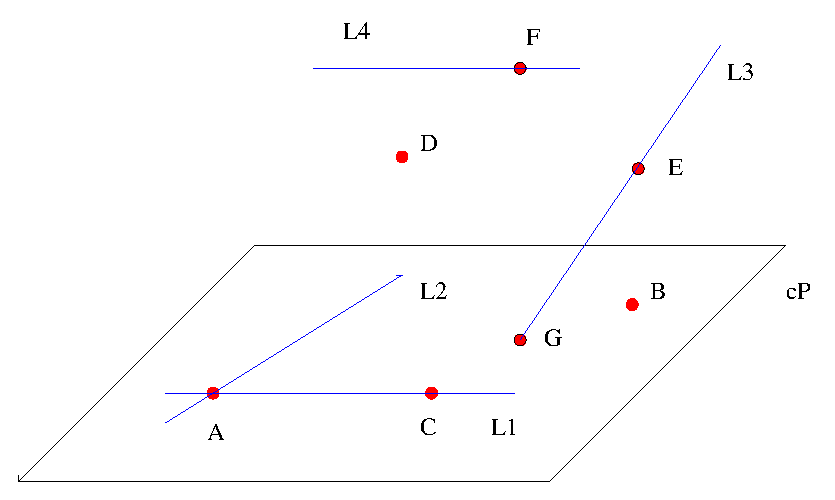
\includegraphics[height=2in]{../../modules/coordinate-systems/pictures/line_plane.eps}
  \caption{Points, lines, and planes}
  \label{fig:points_lines_planes}
\end{figure}
%
\end{frame}
%\begin{frame}
 \frametitle{Distance}

\begin{itemize}
 \item Euclidean Plane: \\
    Through a point $P$ outside a line $L$\\ there passes at most one line $\ell$ parallel to $L$
  \item<2-> Distance - Primordial concept \\
      Quantifies/Measures how close/far apart are any two points \\
      $$d(A,B) = |AB|$$
  \item<3-> Measures of angles $\to$ Perpendicularity
      \begin{itemize}
	\item Line and Line
        \item Line and Plane
        \item Plane and Plane
      \end{itemize}
  \end{itemize}

\end{frame}
%\begin{frame}
%
\begin{figure}[h]
  \psfrag{cP1}{$\mathcal{P}_1$}
  \psfrag{cP2}{$\mathcal{P}_2$}
  \psfrag{L1}{$L_1$}
  \psfrag{L2}{$L_2$}
  \psfrag{L}{$L$}  
  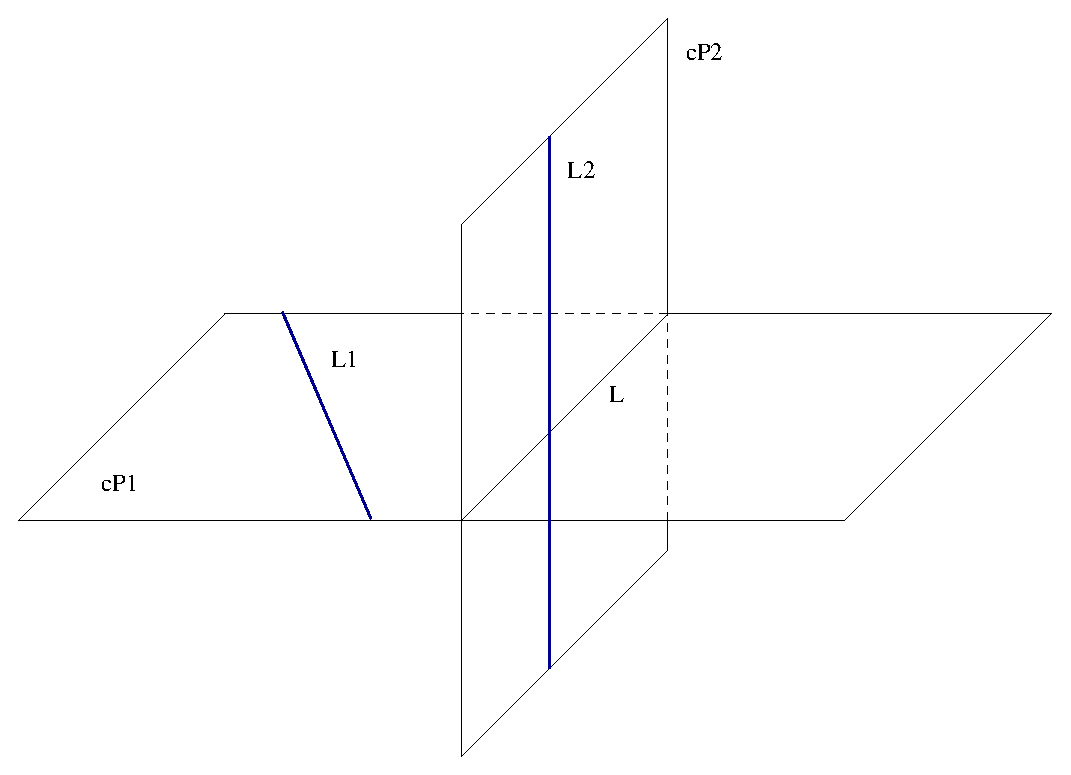
\includegraphics[height=2in]{./images/perpendicularity.eps}
  %\caption{Perpendicularity}
  \label{fig:perpendicularity}
\end{figure}
%
\begin{itemize}
%
\item The planes $\mathcal{P}_1$ and $\mathcal{P}_2$ are perpendicular on each other;
%
\item The lines $L_2$ and $L$ are coplanar and perpendicular on each other;
%
\item The lines $L_1$ and $L_2$ are skew but perpendicular on each other;
%
\item The lines $L_1$ and $L$ are coplanar and not perpendicular;
%
\item The line $L_2$ is perpendicular to the plane $\mathcal{P}_1$;
%
\item The line $L_1$ is not perpendicular to the plane $\mathcal{P}_2$.
\end{itemize}

\end{frame}
%%\begin{comment}
\begin{frame}
\frametitle{Rectangular/Cartesian Coordinates}
\begin{columns}
\column[t]{0.3\textwidth}
\psset{xunit=0.7cm, yunit=0.7cm}
\begin{pspicture}(-0.5 ,-2)(4.5, 4)
\fcBoundingBox{-0.5}{-2}{4.5}{4}
\tiny
\uncover<3->{
\fcLineIIId{[0 0 0]}{[3 0 0]}
\fcLineIIId{[0 0 0]}{[0 3 0]}
\fcLineIIId{[0 0 0]}{[0 0 3]}
}
\uncover<4->{
\fcLineIIId[arrows=->]{[0 0 0]}{[3 0 0]}
\fcLineIIId[arrows=->]{[0 0 0]}{[0 3 0]}
\fcLineIIId[arrows=->]{[0 0 0]}{[0 0 3]}
}
\uncover<5->{
\fcPutIIId[t]{[3 0 0]}{\alertNoH{5}{$x$}}
\fcPutIIId[lb]{[0 3 0]}{\alertNoH{5}{$y$}}
\fcPutIIId[b]{[0 0 3]}{\alertNoH{5}{$z$}}
}
\uncover<2->{ %
\fcPutIIId[r]{[0 0 0]}{$O~~~$} %
\fcDotIIId[linecolor=black]{[0 0 0]} %
}
\end{pspicture}


\vfill
\column{0.7\textwidth}
\begin{itemize}
\item<1-> A Cartesian coordinate system is given by fixing:
\begin{itemize}
\item<2-> a point $O$ (called the origin),
\item<3-> 3 pairwise perpendicular lines intersecting at the origin,
\item<4-> a direction in each of the coordinate axis.
\end{itemize}
\item<5-> The three lines are labeled as $x$-axis, $y$-axis and $z$-axis.
\end{itemize}

\vskip 3cm
\end{columns}


%
\end{frame}

\begin{frame}
\frametitle{Rectangular/Cartesian Coordinates}
\begin{columns}
\column[t]{0.3\textwidth}
\psset{xunit=0.7cm, yunit=0.7cm}
\begin{pspicture}(-0.5 ,-2)(4.5, 4)
\fcBoundingBox{-0.5}{-2}{4.5}{4}
\tiny
\renewcommand{\fcScreen}{[-1 1.1 -0.5] 0}
\fcAxesIIId{3}{3}{3}
\fcPutIIId[r]{[0 0 0]}{$O~$}
\fcPutIIId[b]{[2.5 2.5 2.8]}{$P(x_P,y_P,z_P)$}
\uncover<9->{
\fcLineIIId[linecolor=gray]{[2.5 2.5 2.5]}{[2.5 2.5 0]}
\fcLineIIId[linecolor=gray]{[2.5 2.5 2.5]}{[2.5 0 2.5]}
\fcLineIIId[linecolor=gray]{[2.5 2.5 2.5]}{[0 2.5 2.5]}
\fcLineIIId[linecolor=gray]{[0 2.5 2.5]}{[0 0 2.5]}
\fcLineIIId[linestyle=dashed, linecolor=gray]{[0 2.5 2.5]}{[0 2.5 0]}
\fcLineIIId[linecolor=gray]{[2.5 0 2.5]}{[0 0 2.5]}
\fcLineIIId[linecolor=gray]{[2.5 0 2.5]}{[2.5 0 0]}
\fcLineIIId[linestyle=dashed, linecolor=gray]{[2.5 2.5 0]}{[0 2.5 0]}
\fcLineIIId[linecolor=gray]{[2.5 2.5 0]}{[2.5 0 0]}%
}%
\fcDotIIId{[2.5 2.5 2.5]}%
\uncover<3-8>{%
\fcPerpendicularIIId{[2.5 2.5 2.5]}{[1 0 0]}{0.3}%
\fcPutIIId[t]{[2.5 0 -0.1]}{$Q$}%
}%
\uncover<4->{\fcPutIIId[t]{[1.25 0 -0.1]}{$x_P$}}%
\uncover<6-8>{%
\fcPerpendicularIIId{[2.5 2.5 2.5]}{[0 1 0]}{0.3}%
\fcPerpendicularIIId{[2.5 2.5 2.5]}{[0 0 1]}{0.3}%
}%
\uncover<6->{%
\fcPutIIId[b]{[0 1.25 0.1]}{$y_P$}%
\fcPutIIId[r]{[0 0 1.25]}{$z_P~~$}%
}
\end{pspicture}


\vfill
\column{0.7\textwidth}
\begin{itemize}
\item<1-> $P$ -point. We assign to it triple $(x_P,y_P,z_P)$.
\item<2-> Assignment will be such that distinct points are assigned distinct triples.
\item<3-> $Q=$ base of perpendicular from $P$ to $x$-axis.
\item<4-> Define $x_P$ as \alertNoH{5}{signed distance b-n $O$ and $Q$}.
\item<5-> Take distance with \alertNoH{5}{$+$ sign if $OQ$ points in direction of $x$-axis, $-$ sign else}.
\item<6-> Definitions of $y_P$, $z_P$ are similar.
\item<7-> $(x_P,y_P,z_P)$ = Cartesian coordinates of $P$. 
\item<8-> $x_P$ is called the $x$-coordinate of $P$,  and so on for other axes.
\item<9-> $(x_P, y_P, z_P)$ = singed lengths of edges of the rectangular box indicated in the picture.
\end{itemize}

\vfill
\end{columns}

\vskip 5cm

\end{frame}
%\end{comment}
%\begin{frame}[label=current]
\frametitle{Euclidean Distance in Coordinates}
\begin{definition}
The distance between the points $A(x_A,y_A,z_A)$ and $B(x_B,y_B,z_B)$ is given by:
\[
d(A,B) = |AB| = \sqrt{(x_B-x_A)^2+(y_B-y_A)^2+(z_B-z_A)^2}
\]
\end{definition}
\begin{columns}
\column{0.4\textwidth}
\psset{xunit=1cm, yunit=1cm}
\begin{pspicture}(-2, -2)(2,2)
\renewcommand{\fcScreen}{[-0.5 1 -0.2] -1}
\tiny
\fcAxesIIId{3}{3}{3}
\fcPolyLineIIId[linecolor=red]{[2.6 1 1][2.6 1.4 1] [3 1.4 1] }
\fcPolyLineIIId[linecolor=red]{[2.8 3.7 1][2.8 3.7 1.360555128] [3 4 1.360555128] }

\fcPolyLineIIId[linestyle=dotted]{ [1 1 1] [1 4 1] [1 4 3]}
\fcLineIIId[linestyle=dotted]{[1 4 1]}{[3 4 1]}
\fcParallelogramHollowIIId{ [1 1 1] }{ [3 1 1] }{ [3 1 3] }
\fcParallelogramHollowIIId{ [1 1 3] }{ [3 1 3] }{ [3 4 3] }
\fcParallelogramHollowIIId{ [3 1 1] }{ [3 4 1] }{ [3 4 3] }
\fcLineIIId[linestyle=dotted]{[1 1 1]}{[3 4 1]}
\fcLineIIId[linestyle=dotted]{[1 1 1]}{[3 4 3]}
\fcPutIIId[t]{[1 1 0.9]}{$A$}
\fcPutIIId[l]{[3 4 3]}{$~~B$}
\fcPutIIId[l]{[3 4 1]}{$~~C$}
\fcPutIIId[t]{[3 1 0.9]}{$D$}

\fcPutIIId[t]{[2 1 0.9]}{$x_B- x_A$}
\fcPutIIId[tl]{[3 2.5 1]}{$~~y_B- y_A$}

\fcPutIIId[l]{[3 4 2]}{$~~z_B- z_A$}
\end{pspicture}
\column{0.6\textwidth}
Motivation. 

Pythagorean theorem for $\triangle ADC$: $|AC|^2 = |AD|^2+|DC|^2$.
Pythagorean theorem for $\triangle ACB$: $|AB|^2 =|AC|^2+ |BC|^2= |AD|^2+|DC|^2+|BC|^2 = (x_B-x_A)^2+(y_B-y_A)^2+(z_B-z_A)^2$.
\end{columns}

%\psfrag{O}{$O$}
%\psfrag{A}{$A$} 
%\psfrag{B}{$B(x_B, y_B, z_B)$}  
%\psfrag{C}{$C(x_B, y_B, z_A)$}    
%\psfrag{x}{$y$} 
%\psfrag{y}{$x$} 
%\psfrag{z}{$z$}     
%\psfrag{dx}{$y_B - y_A$}
%\psfrag{dy}{$x_B - x_A$}
%\psfrag{dz}{$z_B - z_A$}  
%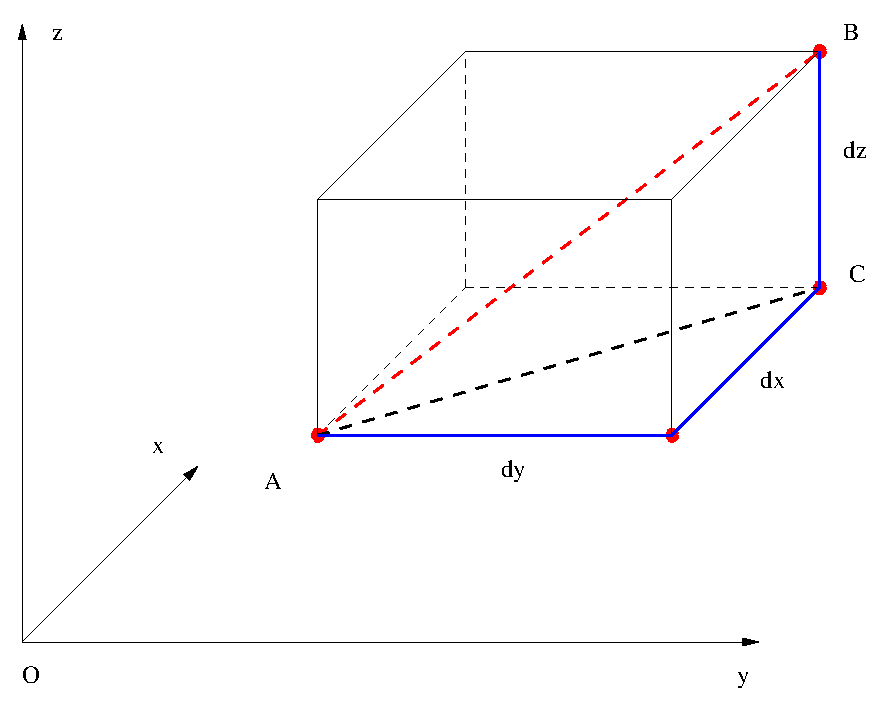
\includegraphics[height=1in]{../../modules/coordinate-systems/pictures/euclidean_distance.eps}
%
%
Example: $P(3,1,2)$ and $Q(1,2,3)$:\pause
%
$$D(P,Q) = \sqrt{(1-3)^2+(2-1)^2+(3-2)^2} = \sqrt{6}\; .$$

\end{frame}
%\begin{frame}
 \frametitle{Change of Coordinates}

  Change in original position and orientation $\to$ new coordinates

\pause

Example:
  \begin{itemize}
   \item Move ahead 1m;
   \item Turn a quarter of a circle to the right.
  \end{itemize}
  
%
\begin{table}[h]
\begin{tabular}{lcr}
  \psfrag{P}{$P(3,1,2)$}
  \psfrag{O}{$O(0,0,0)$}  
  \psfrag{x}{$x=3$} 
  \psfrag{y}{$y=1$} 
  \psfrag{z}{$z=2$}     
  \psfrag{A}{$Ox$}
  \psfrag{L}{$Oy$}
  \psfrag{U}{$Oz$}  
  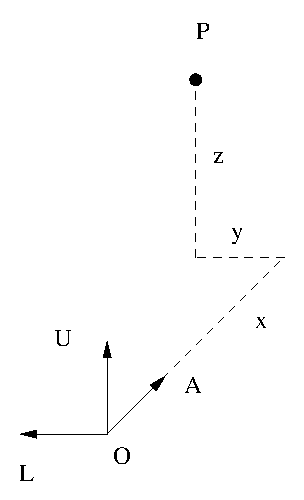
\includegraphics[height=2in]{../../modules/coordinate-systems/pictures/projector.eps}
%
& \hspace{2cm} &
%
\psfrag{P}{$P$}
  \psfrag{Op}{$O'$} 
  \psfrag{O}{$O$}  
  \psfrag{L}{$L$}
  \psfrag{U}{$U$}   
  \psfrag{xp}{$x'=-1$} 
  \psfrag{yp}{$y'=2$} 
  \psfrag{zp}{$z'=2$}     
  \psfrag{Ap}{$A'$}
  \psfrag{Lp}{$L'$}
  \psfrag{Up}{$U'$}  
  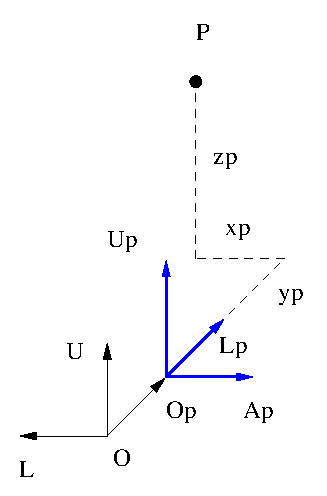
\includegraphics[height=2in]{../../modules/coordinate-systems/pictures/new_frame.eps}
%
\end{tabular}
  \end{table}
%  
%
\pause  
New coordinates of projector: $P \to (x',y',z') = (-1,2,2)$
\end{frame}

\begin{frame}
\frametitle{General formula for this change of coordinates}
%
\begin{table}[h]
\begin{tabular}{lcr}
  \psfrag{P}{$P(x,y,z)$}
  \psfrag{O}{$O(0,0,0)$}  
  \psfrag{x}{$x$} 
  \psfrag{y}{$y$} 
  \psfrag{z}{$z$}     
  \psfrag{A}{$Ox$}
  \psfrag{L}{$Oy$}
  \psfrag{U}{$Oz$}  
  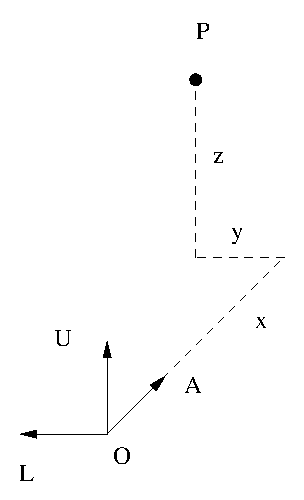
\includegraphics[height=2in]{../../modules/coordinate-systems/pictures/projector.eps}
%
& \hspace{2cm} &
%
\psfrag{P}{$P(x', y', z')$}
  \psfrag{Op}{$O'$} 
  \psfrag{O}{$O$}  
  \psfrag{L}{$L$}
  \psfrag{U}{$U$}   
  \psfrag{xp}{$x'=-y$} 
  \psfrag{yp}{$y'=x-1$} 
  \psfrag{zp}{$z'=z$}     
  \psfrag{Ap}{$A'$}
  \psfrag{Lp}{$L'$}
  \psfrag{Up}{$U'$}  
  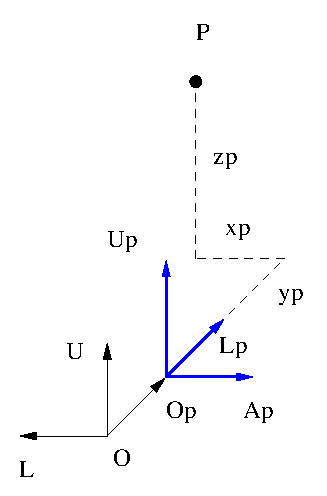
\includegraphics[height=2in]{../../modules/coordinate-systems/pictures/new_frame.eps}
%
\end{tabular}
  \end{table}
%  

\begin{eqnarray*}
 x' = & -y \\
 y' = & x-1 \\
 z' = & z
\end{eqnarray*}
%
Example $Q(x=1,y=2,z=3) \leftrightarrow Q(x'=-2, y'=0,z'=3)$

\end{frame}



\begin{frame}
 \frametitle{Fundamental Philosophy}
  $P(3,1,2)$ and $Q(1,2,3)$ in $(x,y,z)-$coordinates

  $P(-1,2,2)$ and $Q(-2,0,3)$ in $(x',y'z')-$coordinates

  Distance in new coordinates:
 \pause
%
$$d_{x',y',z'}(P,Q) = \sqrt{(-2+1)^2+(0-2)^2+(3-2)^2} = \sqrt{6} = d_{x,y,z}(P,Q)$$

Fundamental Philosophy:\pause
\begin{itemize}
 \item Space doesn't come with coordinates
  \item Natural concepts (such of distance) are independent of coordinates
  \item If a natural concept is defined using coordinates, \\
          the result does not depend on the chosen coordinate system.
\end{itemize}


\end{frame}
%\begin{frame}
  \frametitle{Sets in Space}

  $X$ subset of a set $Y$:

  $$X = \{ A \text{ in } Y | A \text{ has property } \mathcal{P} \} \subset Y$$

\pause
Examples  (Fixed point $Q$, fixed $r>0$):

$$X = \{ A \text{ in Space } | d(A,Q) = r \} = S_r(Q)\; ,$$
\pause Sphere of radius $r$ centered at $Q$.\pause

$$B_r(Q) = \{ A \text{ in Space } | d(A,Q) <r \} \; ,$$
\pause  Open ball of radius $r$ centered at $Q$. \pause

$$\overline{B}_r(Q) = \{ A \text{ in Space } | d(A,Q) \leqslant r\} \; ,$$
\pause  Closed ball of radius $r$ centered at $Q$.

\end{frame}
%\begin{frame}
 \frametitle{Equation(s) of Subsets}

  $$X = \{ (x,y,z) | x,y,z \text{ satisfy certain relation(s) } \} \; .$$

\pause
Examples:

$\{(x,y,z) | x^2+y^2+z^2 = 1\}$:

\pause
sphere of radius $r=1$ centered at the origin $(0,0,0)$

Also refered to as: sphere $x^2+y^2+z^2 = 1$

\pause
\medskip

$\{ (x,y,z) | x=0 \}$: coordinate Left-Up plane

\pause
\medskip

$\{ (x,y,z) | x=0 \text{ and } y=0 \}$:

intersection of coordinate planes $\rightarrow$ coordinate axis

\pause
\medskip

Can be given by only one equation:

$x^2+y^2 = 0$ $\rightarrow$ $x=0$,$y=0$, and $z$ arbitrary $\rightarrow$

vertical axis above $(0,0)$ in $(x,y)-$plane

\pause
\medskip

Important: Equations in Plane vs. Space.

\end{frame}
%\begin{frame}
 \frametitle{Recognizing Spheres from Equations}

  $Q(x_0,y_0,z_0)$, $r>0$, $A(x,y,z)$. Remark: $d(A,Q) = r \longleftrightarrow d^2(A,Q) = r^2$

$$S_r(Q): \quad (x-x_0)^2+(y-y_0)^2+(z-z_0)^2 = r^2$$

\pause
Example:
$$(x-2)^2+(y-0)^2+(z+1)^2=3^2$$
%
$$x^2+y^2+z^2 -4x + 2z -4=0$$

\pause
\begin{itemize}
 \item no mixed terms $xy$, $xz$, or $yz$;
 \item quadratic terms $x^2$, $y^2$, and $z^2$ with the same coefficient.
\end{itemize}

\pause
Examples:
$$x^2+y^2+z^2-4x+2y=0$$
%
\pause
Complete the square:
%
$$(x-2)^2 + (y+1)^2 +z^2 = 5$$
%
Sphere of radius $\sqrt{5}$ centered at $(2,-1,0)$.

\pause
How about $x^2+y^2+z^2 - 4x+2y = -6$? \pause Passes both tests, but ...
%
$$(x-2)^2 + (y+1)^2 +z^2 = -1$$
%
is impossible! No such points, set is empty.

\end{frame}

\section{Polar Coordinates}
% begin module polar-intro
\begin{frame}
\frametitle{Polar Coordinates}
\begin{itemize}
\item  The polar coordinates system is an alternative to the Cartesian coordinates system.
%\item  Instead of specifying horizontal distance and vertical distance, we specify angle and distance from the origin.
\item  Choose a point in the plane called $O$ (the origin).
\item  Draw a ray starting at $O$ called the polar axis.  This ray is usually drawn horizontally to the right.
\end{itemize}
\begin{columns}[c]
\column{.5\textwidth}
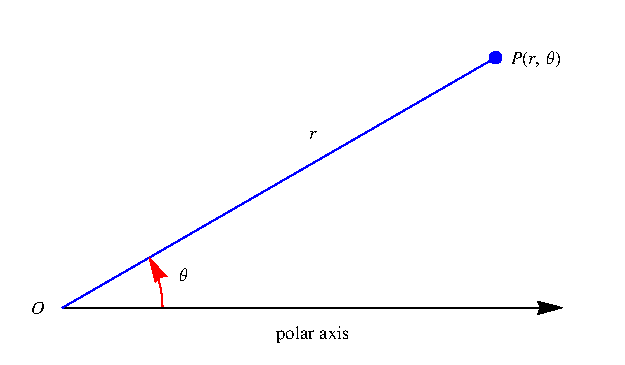
\includegraphics[height=4cm]{polar-curves/pictures/11-03-polar.pdf}%
\column{.5\textwidth}
\begin{itemize}
\item  Let $P$ be a point in the plane.
\item  Let $\theta$ denote the angle between the polar axis and the line $OP$.
\item  Let $r$ denote the length of the line $OP$.
\item  Then $P$ is represented by the ordered pair $(r, \theta )$.
\end{itemize}
\end{columns}
\end{frame}
% end module polar-intro

% begin module polar-questions
\begin{frame}
\begin{enumerate}
\item<1-| alert@2>  What if $\theta$ is negative?
\item<1-| alert@3>  What if $r$ is negative?
\item<1-| alert@4>  What if $r$ is $0$?
\end{enumerate}
\begin{columns}[c]
\column{.5\textwidth}
\uncover<2->{
\psset{xunit=2cm, yunit=2cm}
\begin{pspicture}(-0.9, -1.2)(2,0.2)
\tiny
%force a boudning box:
%\psline[linecolor=red!1](-0.1, -0.1)(-0.21,0.2)
%\psline[linecolor=red!1](1.1, 0.6)(1.1,0.61)
\fcFullDotBlue{0}{0}

%Calculator input: plotCurve{}(1/10 \cos{}t, 1/10 \sin{}t, 0, -3/4 \pi)
\parametricplot[arrows=->, linecolor=\fcColorGraph, plotpoints=100]{0} {-2.35619} {t 57.29578 mul cos 0.3000000 mul t 57.29578 mul sin 0.3000000 mul }
\rput[t] (0,-0.1){$O$}
\rput[l](0.3, -0.2){$\theta=-\frac{3\pi}{4}$}

\psline{->}(0,0)(2,0)
\psline[linecolor=blue](0,0)(-0.707106781, -0.707106781)
\fcFullDotBlue{-0.707106781}{-0.707106781}
\rput[tl](-0.6, -0.7){$\begin{array}{l}(r,\theta)=\left(1, -\frac{3\pi}{4}\right)\\ (x,y)=\left(-\frac{\sqrt{2}}2, -\frac{\sqrt{2}}2 \right) \end{array}$}
\end{pspicture}
}

\uncover<3->{
\psset{xunit=2cm, yunit=2cm}
\begin{pspicture}(-0.9, -1.5)(1.7,0.8)
\tiny
%force a boudning box:
%\psline[linecolor=red!1](-0.1, -0.1)(-0.21,0.2)
%\psline[linecolor=red!1](1.1, 0.6)(1.1,0.61)
\fcFullDotBlue{0}{0}

\parametricplot[arrows=->, linecolor=\fcColorGraph, plotpoints=100]{0} {0.523598776 } {t 57.29578 mul cos 0.3000000 mul t 57.29578 mul sin 0.3000000 mul }
\parametricplot[arrows=->, linecolor=brown, plotpoints=100]{0} {3.665191429 } {t 57.29578 mul cos 0.25 mul t 57.29578 mul sin 0.25 mul }

\rput[t] (0,-0.1){$O$}

\psline{->}(0,0)(1,0)
\psline[linecolor=blue](0,0)(0.866025404, 0.5)
\fcFullDotBlue{0.866025404}{0.5}
\rput[tl](-0.75, -0.5){
$(-r, \theta)$
}
\fcFullDotBlue{-0.866025404}{-0.5}
\psline[linecolor=blue, linestyle=dashed](0,0) (-0.866025404,-0.5)
\rput[tl](0.6, 0.7){$(r, \theta) $}
\end{pspicture}
}
%\ \uncover<2->{%
%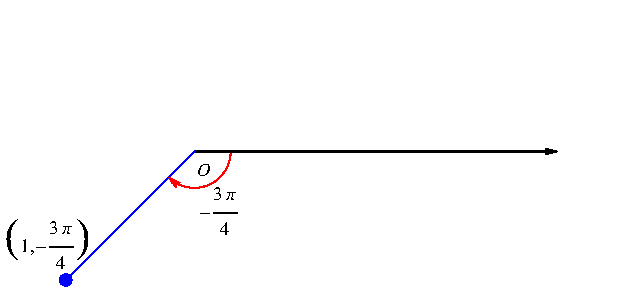
\includegraphics[height=3cm]{polar-curves/pictures/11-03-ex1b.pdf}%
%}%
%\ \uncover<3->{%
%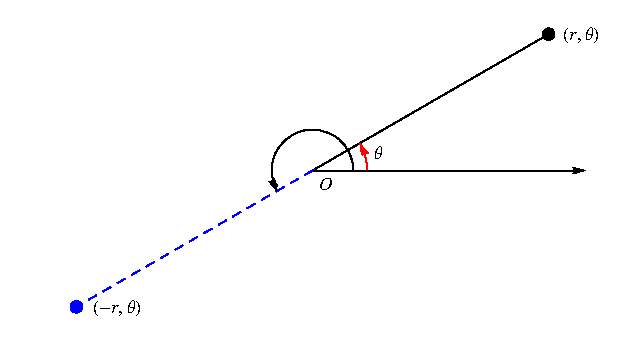
\includegraphics[height=3cm]{polar-curves/pictures/11-03-negativer.pdf}%
%}%
\column{.5\textwidth}
\begin{enumerate}
\item<2-| alert@2>  Positive angles $\theta$ are measured in the counterclockwise direction from $O$.  Negative angles are measured in the clockwise direction.
\item<3-| alert@3>  Points with polar coordinates $(-r, \theta)$ and $(r, \theta)$ lie on the same line through $O$ and at the same distance from $O$, but on opposite sides.
\item<4-| alert@4>  If $r = 0$, then $(r, \theta) = P = O$ for all values of $\theta$.
\end{enumerate}
\end{columns}
\end{frame}
% end module polar-questions

% begin module polar-many-representations
\begin{frame}
\begin{columns}[T]
\column{.5\textwidth}
\uncover<1->{
\psset{xunit=2cm, yunit=2cm}
\begin{pspicture}(-0.9, -1.1)(2,0.5)
\tiny
%force a boudning box:
%\psline[linecolor=red!1](-0.1, -0.1)(-0.21,0.2)
%\psline[linecolor=red!1](1.1, 0.6)(1.1,0.61)
\fcFullDotBlue{0}{0}

%Calculator input: plotCurve{}(1/10 \cos{}t, 1/10 \sin{}t, 0, -3/4 \pi)
\parametricplot[arrows=->, linecolor=\fcColorGraph, plotpoints=100]{0} {3.926990817} {t 57.29578 mul cos 0.3000000 mul t 57.29578 mul sin 0.3000000 mul }
\rput[t] (0,-0.1){$O$}
\rput[l](0.3, 0.3){$\theta=\frac{5\pi}{4}$}

\psline{->}(0,0)(2,0)
\psline[linecolor=blue](0,0)(-0.707106781, -0.707106781)
\fcFullDotBlue{-0.707106781}{-0.707106781}
\rput[tl](-0.6, -0.7){$(r,\theta)=\left(1, \frac{5\pi}{4}\right)$}
\end{pspicture}
}
\uncover<2->{
\psset{xunit=2cm, yunit=2cm}
\begin{pspicture}(-0.9, -1.1)(2,0.5)
\tiny
%force a boudning box:
%\psline[linecolor=red!1](-0.1, -0.1)(-0.21,0.2)
\psline[linecolor=red!1](1.1, 0.5)(1.1,0.51)
\fcFullDotBlue{0}{0}

%Calculator input: plotCurve{}(1/10 \cos{}t, 1/10 \sin{}t, 0, -3/4 \pi)
\parametricplot[arrows=->, linecolor=\fcColorGraph, plotpoints=100]{0} {-2.35619} {t 57.29578 mul cos 0.3000000 mul t 57.29578 mul sin 0.3000000 mul }
\rput[t] (0,-0.1){$O$}
\rput[l](0.3, -0.2){$\theta=-\frac{3\pi}{4}$}

\psline{->}(0,0)(2,0)
\psline[linecolor=blue](0,0)(-0.707106781, -0.707106781)
\fcFullDotBlue{-0.707106781}{-0.707106781}
\rput[tl](-0.6, -0.7){$(r,\theta)=\left(1, -\frac{3\pi}{4}\right)$}
\end{pspicture}
}

%\ \uncover<1->{%
%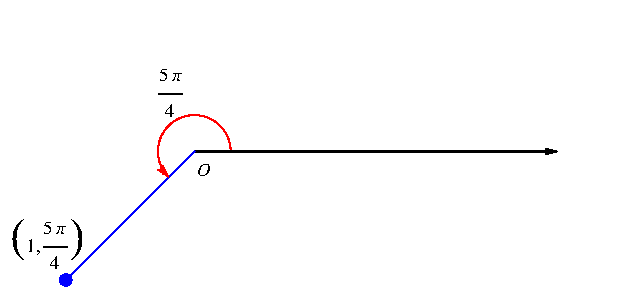
\includegraphics[height=3cm]{polar-curves/pictures/11-03-ex1a.pdf}%
%}%

%\ \uncover<2->{%
%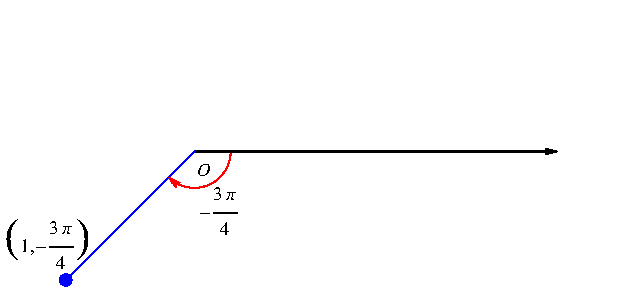
\includegraphics[height=3cm]{polar-curves/pictures/11-03-ex1b.pdf}%
%}%
\column{.5\textwidth}
\uncover<3->{
\psset{xunit=2cm, yunit=2cm}
\begin{pspicture}(-0.9, -1.1)(2,0.5)
\tiny
%force a boudning box:
%\psline[linecolor=red!1](-0.1, -0.1)(-0.21,0.2)
%\psline[linecolor=red!1](1.1, 0.6)(1.1,0.61)
\fcFullDotBlue{0}{0}

%Calculator input: plotCurve{}(1/50 t \cos{}t+3/20 \cos{}t, 1/50 t \sin{}t+3/20 \sin{}t, 0, 13/4 \pi)
\parametricplot[arrows=->, linecolor=\fcColorGraph, plotpoints=400] {0} {10.2102} {t 57.29578 mul cos 0.1500000 mul t 57.29578 mul cos t mul 0.0200000 mul add t 57.29578 mul sin 0.1500000 mul t 57.29578 mul sin t mul 0.0200000 mul add }

\rput[t] (0,-0.1){$O$}
\rput[l](0.3, 0.3){$\theta=\frac{13\pi}{4}$}

\psline{->}(0,0)(2,0)
\psline[linecolor=blue](0,0)(-0.707106781, -0.707106781)
\fcFullDotBlue{-0.707106781}{-0.707106781}
\rput[tl](-0.6, -0.7){$(r,\theta)=\left(1, \frac{13\pi}{4}\right)$}
\end{pspicture}
}

\uncover<4->{
\psset{xunit=2cm, yunit=2cm}
\begin{pspicture}(-0.9, -1.1)(2,0.5)
\tiny
%force a boudning box:
%\psline[linecolor=red!1](-0.1, -0.1)(-0.21,0.2)
\psline[linecolor=red!1](1.1, 0.5)(1.1,0.51)
\fcFullDotBlue{0}{0}

%Calculator input: plotCurve{}(1/10 \cos{}t, 1/10 \sin{}t, 0, -3/4 \pi)
\parametricplot[arrows=->, linecolor=\fcColorGraph, plotpoints=100]{0} {0.785398163} {t 57.29578 mul cos 0.3000000 mul t 57.29578 mul sin 0.3000000 mul }
\rput[t] (0,-0.1){$O$}
\rput[l](0.35, 0.15){$\theta=\frac{\pi}{4}$}

\psline{->}(0,0)(2,0)
\psline[linecolor=blue](0,0)(-0.707106781, -0.707106781)
\fcFullDotBlue{-0.707106781}{-0.707106781}
\psline[linestyle=dashed](0,0)(0.707106781, 0.707106781)
\fcFullDotBlack{0.707106781}{0.707106781}
\rput[tl](-0.6, -0.7){$(r,\theta)=\left(-1, \frac{\pi}{4}\right)$}
\end{pspicture}
}
%\ \uncover<3->{%
%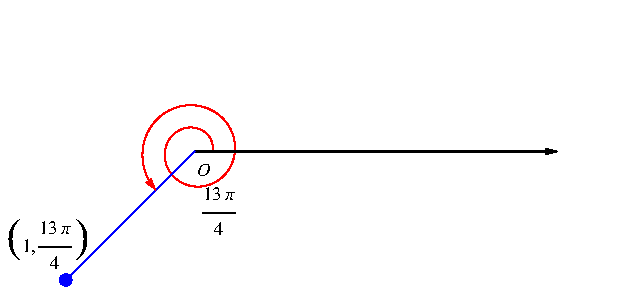
\includegraphics[height=3cm]{polar-curves/pictures/11-03-ex1c.pdf}%
%}%

%\ \uncover<4->{%
%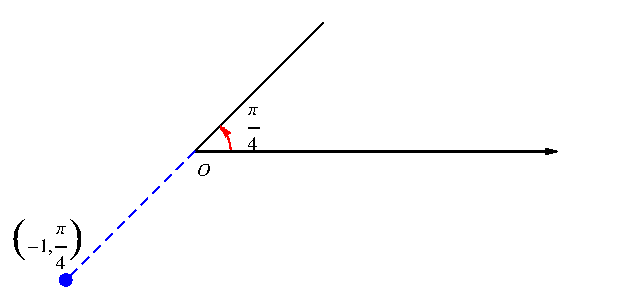
\includegraphics[height=3cm]{polar-curves/pictures/11-03-ex1d.pdf}%
%}%
\end{columns}
\begin{itemize}
\item  There are many ways to represent the same point.
\item<2-| alert@2>  We could use a negative $\theta$.
\item<3-| alert@3>  We could go around more than once.
\item<4-| alert@4>  We could use a negative $r$.
\end{itemize}
\end{frame}
% end module polar-many-representations

%begin module polar-two-points-coincide-iff
\begin{frame}
\begin{itemize}
\item Let $P_1$ be point  with polar coordinates $(r_1, \theta_1)$.
\item Let $P_2$ be point  with polar coordinates $(r_2, \theta_2)$.
\end{itemize}

\uncover<2->{
\begin{observation}
$P_1$ coincides with $P_2$ if one of the three mutually exclusive possibilities holds:
\begin{itemize}
\item<alert@3> $r_1=r_2\neq 0$ and $\theta_2=\theta_1+2k\pi, k\in \mathbb Z $,
\item<alert@4> $r_1=-r_2\neq 0$ and $\theta_2=\theta_1+(2k+1)\pi, k\in \mathbb Z$,
\item $r_1=r_2=0 $ and $\theta$ is arbitrary.
\end{itemize}
\end{observation}
}
\begin{columns}
\column{.5\textwidth}
\only<3>{
\psset{xunit=2cm, yunit=2cm}
\begin{pspicture}(-0.9, -1.1)(2,0.75) 
\tiny 
%force a boudning box:
%\psline[linecolor=red!1](-0.1, -0.1)(-0.21,0.2)
%\psline[linecolor=red!1](1.1, 0.6)(1.1,0.61)
\psFullDotBlue{0}{0}

%Calculator input: plotCurve{}(1/10 \cos{}t, 1/10 \sin{}t, 0, -3/4 \pi)
\parametricplot[arrows=->, linecolor=\psColorGraph, plotpoints=100]{0} {3.926990817} {t 57.29578 mul cos 0.3000000 mul t 57.29578 mul sin 0.3000000 mul }
\rput[t] (0,-0.1){$O$}
\rput[l](0.3, 0.3){$\theta_1$}

\psline{->}(0,0)(2,0)
\psline[linecolor=blue](0,0)(-0.707106781, -0.707106781)
\psFullDotBlue{-0.707106781}{-0.707106781}
\rput[tl](-0.6, -0.7){$(r_1,\theta_1)$}
\end{pspicture} 
}
\uncover<4>{
\psset{xunit=2cm, yunit=2cm}
\begin{pspicture}(-0.9, -1.1)(2,0.75) 
\tiny 
%force a boudning box:
%\psline[linecolor=red!1](-0.1, -0.1)(-0.21,0.2)
\psline[linecolor=red!1](1.1, 0.5)(1.1,0.51)
\psFullDotBlue{0}{0}

%Calculator input: plotCurve{}(1/10 \cos{}t, 1/10 \sin{}t, 0, -3/4 \pi)
\parametricplot[arrows=->, linecolor=\psColorGraph, plotpoints=100]{0} {-2.35619} {t 57.29578 mul cos 0.3000000 mul t 57.29578 mul sin 0.3000000 mul }
\rput[t] (0,-0.1){$O$}
\rput[l](0.3, -0.2){$\theta_1$}

\psline{->}(0,0)(2,0)
\psline[linecolor=blue](0,0)(-0.707106781, -0.707106781)
\psFullDotBlue{-0.707106781}{-0.707106781}
\rput[tl](-0.6, -0.7){$(r_1,\theta_1)$}
\end{pspicture} 
}

%\ \uncover<1->{%
%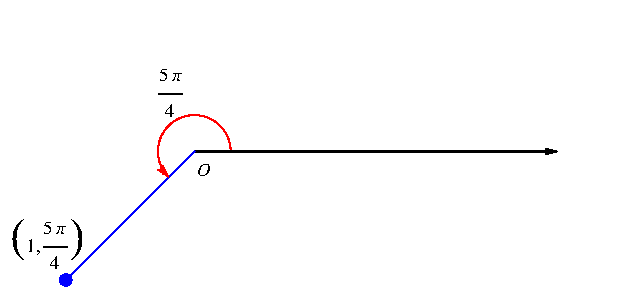
\includegraphics[height=3cm]{polar-curves/pictures/11-03-ex1a.pdf}%
%}%

%\ \uncover<2->{%
%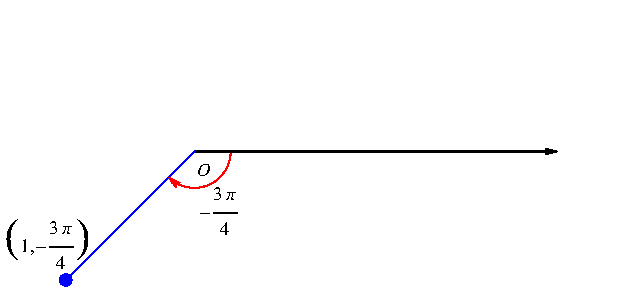
\includegraphics[height=3cm]{polar-curves/pictures/11-03-ex1b.pdf}%
%}%

\vspace{2cm}
\column{.5\textwidth}
\only<3>{
\psset{xunit=2cm, yunit=2cm}
\begin{pspicture}(-0.9, -1.1)(2,0.75) 
\tiny 
%force a boudning box:
%\psline[linecolor=red!1](-0.1, -0.1)(-0.21,0.2)
%\psline[linecolor=red!1](1.1, 0.6)(1.1,0.61)
\psFullDotBlue{0}{0}

%Calculator input: plotCurve{}(1/50 t \cos{}t+3/20 \cos{}t, 1/50 t \sin{}t+3/20 \sin{}t, 0, 13/4 \pi)
\parametricplot[arrows=->, linecolor=\psColorGraph, plotpoints=400] {0} {10.2102} {t 57.29578 mul cos 0.1500000 mul t 57.29578 mul cos t mul 0.0200000 mul add t 57.29578 mul sin 0.1500000 mul t 57.29578 mul sin t mul 0.0200000 mul add }

\rput[t] (0,-0.1){$O$}
\rput[l](0.3, 0.3){$\theta_2=\theta_1+2\pi$}

\psline{->}(0,0)(2,0)
\psline[linecolor=blue](0,0)(-0.707106781, -0.707106781)
\psFullDotBlue{-0.707106781}{-0.707106781}
\rput[tl](-0.6, -0.7){$(r_2, \theta_2)=(r_1,\theta_1+2\pi)$}
\end{pspicture} 
}

\uncover<4>{
\psset{xunit=2cm, yunit=2cm}
\begin{pspicture}(-0.9, -1.1)(2,0.75) 
\tiny 
%force a boudning box:
%\psline[linecolor=red!1](-0.1, -0.1)(-0.21,0.2)
\psline[linecolor=red!1](1.1, 0.5)(1.1,0.51)
\psFullDotBlue{0}{0}

%Calculator input: plotCurve{}(1/10 \cos{}t, 1/10 \sin{}t, 0, -3/4 \pi)
\parametricplot[arrows=->, linecolor=\psColorGraph, plotpoints=100]{0} {0.785398163} {t 57.29578 mul cos 0.3000000 mul t 57.29578 mul sin 0.3000000 mul }
\rput[t] (0,-0.1){$O$}
\rput[l](0.35, 0.15){$\theta_2=\theta_1+\pi$}

\psline{->}(0,0)(2,0)
\psline[linecolor=blue](0,0)(-0.707106781, -0.707106781)
\psFullDotBlue{-0.707106781}{-0.707106781}
\psline[linestyle=dashed](0,0)(0.707106781, 0.707106781)
\psFullDotBlack{0.707106781}{0.707106781}
\rput[tl](-0.6, -0.7){$(r_2, \theta_2)=(-r_1,\theta_1+\pi)$}
\end{pspicture} 
}
%\ \uncover<3->{%
%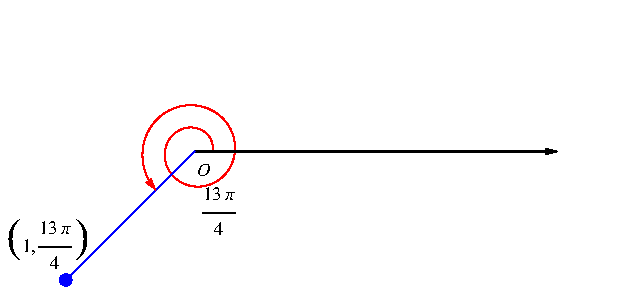
\includegraphics[height=3cm]{polar-curves/pictures/11-03-ex1c.pdf}%
%}%

%\ \uncover<4->{%
%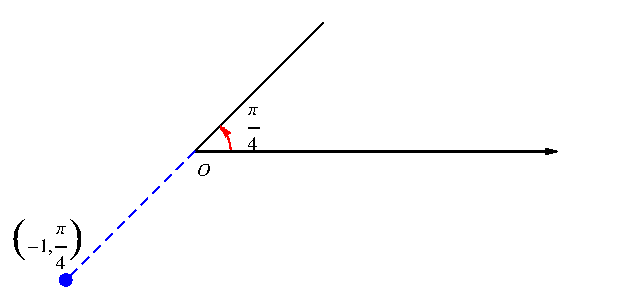
\includegraphics[height=3cm]{polar-curves/pictures/11-03-ex1d.pdf}%
%}%

\vspace{2cm}
\end{columns}
\end{frame}
%end module polar-two-points-coincide-iff
% begin module polar-to-cartesian
\begin{frame}
\begin{itemize}
\item  How do we go from polar coordinates to Cartesian coordinates?
\item<2->  Suppose a point has polar coordinates $(r, \theta )$ and Cartesian coordinates $(x,y)$.
\item<8->  How do we go from Cartesian coordinates to polar coordinates?
\end{itemize}
\begin{columns}[c]
\column{0.5\textwidth}
\psset{xunit=4cm, yunit=4cm}
\begin{pspicture}(-0.2, -0.2)(1.400000,0.9)
\tiny
%force a boudning box:
\psline[linecolor=red!1](-0.1, -0.1)(-0.21,0.2)
\psline[linecolor=red!1](1.1, 0.6)(1.1,0.61)
\psaxes[arrows=<->, ticks=none, labels=none](0,0)(-0.2, -0.2)(1, 0.8)
\rput(-0.03, 0.8){$y$}
\rput(1,-0.03){$x$}
%\fcAxesStandard{-0.2}{-0.2}{1}{0.8}

%Calculator input: plotCurve{}(1/5 \cos{}t, 1/5 \sin{}t, 0, 1/6 \pi)
\parametricplot[arrows=->, linecolor=red, plotpoints=1000] {0}{0.523599}{t 57.29578 mul cos 0.2 mul t 57.29578 mul sin 0.2 mul }
\psline[linecolor=blue](0,0)(0.866025404, 0.5)
\rput(0.22, 0.06){$\theta$}

\fcFullDotBlue{0.866025404}{0.5}
\psline(0.866025404,0.5)(0.866025404,0)
\psline(0.846025404, 0)(0.846025404, 0.02)(0.866025404, 0.02)
\rput[l](0.9, 0.5){$P(r,\theta) =(x,y)$}

\uncover<6>{
\psline{<-}(0.89, 0)(0.89, 0.2)
}
\uncover<6->{
\rput(0.89,0.25){$\alert<6,10>{y}$}
}
\uncover<6>{
\psline{->}(0.89, 0.3)(0.89, 0.5)
}
\uncover<4>{
\psline{<-}(0, -0.02)(0.385, -0.02)
}
\uncover<4->{
\rput(0.435,-0.02){$\alert<4,10>{x}$}
}
\uncover<4>{
\psline{->}(0.485, -0.02)(0.866025404, -0.02)
}
\rput[tr](-0.03, -0.03){$O$}
\rput(0.4, 0.3){$\alert<4,6,9,10>{r}$}
\end{pspicture}
%\ \uncover<2->{%
%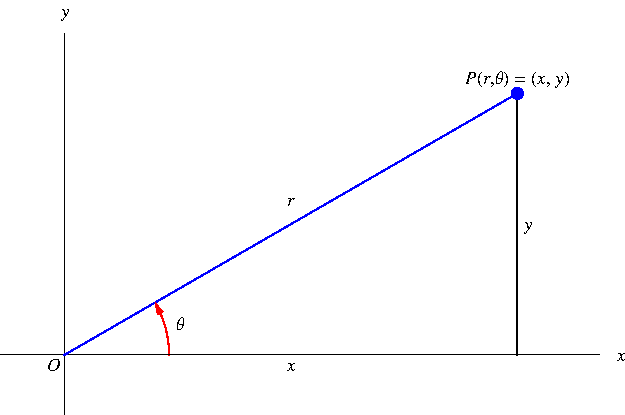
\includegraphics[height=5cm]{polar-curves/pictures/11-03-conversion.pdf}%
%}%
\column{.5\textwidth}
$
\renewcommand{\arraystretch}{1.5}
\begin{array}{rcl}
\alert<7>{x} &\alert<7>{=}&\uncover<7->{\alert<7>{r\cos \theta} } \\
\alert<7>{y}&\alert<7>{=}& \uncover<7->{\alert<7>{r\sin \theta}} \\\hline
\uncover<3->{\alert<3,4,7>{\cos\theta}} & \uncover<3->{\alert<3,4,7>{=}} &\displaystyle \uncover<4->{\alert<4,7>{\frac{x}{r} }} \\
\uncover<3->{\alert<5,6,7>{\sin \theta}} &\uncover<3->{ \alert<5,6,7>{= }} & \displaystyle \uncover<6->{\alert<6,7>{\frac{y}{r}}}\\
\uncover<9->{\alert<handout:0| 9-10>{r^2} &\alert<9,10>{=}& \uncover<10->{\alert<10>{x^2 + y^2}}}\\\hline
\alert<8,9,10,11>{ r}&\alert<8,9,10,11>{=}&\uncover<11->{\alert<11>{ \sqrt{x^2+y^2}}} \\
\alert<12,13>{\theta} &\alert<12,13>{=}&  
\uncover<13->{\alert<13>{\arcsin \left(\frac{y}{r}\right)  \text{\quad if } x>0}}\\ 
\uncover<13->{
&\alert<13>{=}&\alert<13>{\arccos \left(\frac{x}{r}\right)  \text{\quad if } y>0}}\\
\uncover<13->{&\alert<13>{=}&\alert<13>{\arctan \left(\frac{y}{x}\right)  \text{\quad if } x>0}}
\end{array}
$


\end{columns}
\end{frame}
% end module polar-to-cartesian

% begin module polar-to-cartesian-ex2
\begin{frame}
\begin{example} 
Convert the point $(\alert<handout:0| 4>{2}, \alert<handout:0| 6>{\frac{\pi}{3}})$ from polar to Cartesian coordinates.
\[
\uncover<2->{%
x = \alert<handout:0| 3-4>{r}\cos \alert<handout:0| 5-6>{\theta} = %
}%
\uncover<3->{%
\alert<handout:0| 3-4>{\uncover<4->{2}}\alert<handout:0| 7-8>{ \cos } \alert<handout:0| 5-8>{\uncover<6->{\frac{\pi}{3}}} %
}%
\uncover<7->{%
= 2\left( \alert<handout:0| 7-8>{\uncover<8->{\frac{ 1}{ 2 } } } \right) \uncover<9->{ = 1}%
}%
\]
\[
\uncover<2->{%
y = r\sin \theta = %
}%
\uncover<10->{%
2\alert<handout:0| 11-12>{\sin \frac{\pi}{3}}%
}%
\uncover<11->{%
= 2\left( \alert<handout:0| 11-12>{ \uncover<12->{ \frac{ \sqrt{ 3 }}{2}}}\right) \uncover<13->{ = \sqrt{3}}%
}%
\]
\uncover<14->{%
Therefore the point with polar coordinates $(2,\frac{\pi}{3})$ has Cartesian coordinates $(1,\sqrt{3})$.
}%
\end{example}
\end{frame}
% end module polar-to-cartesian-ex2

% begin module polar-to-cartesian-ex3
\begin{frame}
\begin{example}
\begin{columns}
\column{0.25\textwidth}
\psset{xunit=0.65cm, yunit=0.65cm}
\begin{pspicture}(-1,-1)(2,2)
\tiny
\fcAxesStandard{-1.5}{-1.5}{1.5}{1.5}
\fcLabels{1.5}{1.5}
\uncover<9->{%
\fcFullDot{1}{-1}%
}%
\uncover<11->{% 
\fcAngleDegrees[arrows=->, linecolor=red]{0}{315}{0.2} { }%
\rput[b](-0.3, 0.2){$\frac{7\pi}{4}$}
\psline(0,0)(1,-1)
}%
\uncover<13->{%
\fcAngleDegrees{0}{-45}{0.4}{}
\rput[t](0.6, -0.2){$-\frac{\pi}{4}$}
}%
\end{pspicture}
\column{0.75\textwidth}
Represent the point with Cartesian coordinates $(1,-1)$ in terms of polar coordinates.
\end{columns}
\begin{columns}
\column{.6\textwidth}
\begin{itemize}
\item<3-| alert@3-4>  Suppose $r$ is positive.
\item<7->  $\tan \theta = -1$ for $\theta = \alert<handout:0| 10>{\frac{3\pi}{4}}, \alert<handout:0| 10-11>{\frac{7\pi}{4}}$, and many other angles.
\item<8-| alert@8-9>  $(1,-1)$ is in the \uncover<9->{fourth} quadrant.
\item<10->  Of the two values above, only \alert<handout:0| 10-11>{$\theta = \uncover<11->{\frac{7\pi}{4}}$} gives a point in the fourth quadrant.
\item<12->  Therefore one possible representation of $(1,-1)$ in polar coordinates is $(\sqrt{2}, 7\pi/4)$.
\item<13->  $(\sqrt{2}, -\pi /4)$ is another.
\end{itemize}
\column{.4\textwidth}
\begin{eqnarray*}
\uncover<2->{%
r%
}%
& \uncover<2->{ = } &%
\uncover<2->{%
\uncover<-3>{\alert<handout:0| 3>{\pm}} \sqrt{x^2+y^2}%
}\\%
& \uncover<5->{ = } &%
\uncover<5->{%
\sqrt{1^2 + (-1)^2}%
}\\% = \sqrt{2}%
& \uncover<5->{ = } &%
\uncover<5->{%
\sqrt{2}%
}\\% = \sqrt{2}%
&&\\
\uncover<2->{%
\tan \theta%
}%
& \uncover<2->{ = } &%
\uncover<2->{%
\frac{y}{x}%
}\\%
& \uncover<6->{ = } &%
\uncover<6->{%
-1%
}\\%
\end{eqnarray*}
\end{columns}
\end{example}
\end{frame}
% end module polar-to-cartesian-ex3

% begin module polar-intersection-ex3
\begin{frame}
\begin{example} %[Example 3, p. 688]
Find all points of intersection of the polar curves $r = \frac{1}{2}$ and $r = \cos (2\theta)$.
\begin{columns}[c]
\column{.4\textwidth}

\psset{xunit=1.8cm, yunit=1.8cm}
\begin{pspicture}(-1.5, -1.5)(1.5,1.5)
\tiny
\fcAxesStandard{-1.4}{-1.4}{1.4}{1.4}
%Calculator command: drawPolar{}(1/2, 0, 2 \pi)
\parametricplot[linecolor=\fcColorGraph, plotpoints=1000, algebraic=false]{0}{6.28319}{ 0.5 t 57.29578 mul cos mul 0.5 t 57.29578 mul sin mul }
%Calculator command: drawPolar{}(\cos{}(2 t), 0, 2 \pi)
\parametricplot[linecolor=\fcColorGraph, plotpoints=1000, algebraic=false]{0}{6.28319}{t 2 mul 57.29578 mul cos t 57.29578 mul cos mul t 2 mul 57.29578 mul cos t 57.29578 mul sin mul }

\rput[tr](-0.8, -0.8){$r=\frac{1}{2}$}
\psline{->}(-0.75, -0.75)(-0.353553391, -0.353553391)
\rput[lt] (0.2, -1){$r=\cos (2\theta)$}

\uncover<4->{
\fcFullDotBlack{0.433013}{0.25}
\fcFullDotBlack{-0.433013}{0.25}
\fcFullDotBlack{-0.433013}{-0.25}
\fcFullDotBlack{0.433013}{-0.25}
}
\uncover<6->{
\fcFullDotBlack{0.25}{0.433013}
\fcFullDotBlack{0.25}{-0.433013}
\fcFullDotBlack{-0.25}{-0.433013}
\fcFullDotBlack{-0.25}{0.433013}
}
\uncover<9>{
\pscircle*[linecolor=red](0.433013,0.25){0.09}
\pscircle*[linecolor=red](-0.433013,0.25){0.09}
\pscircle*[linecolor=red](-0.433013,-0.25){0.09}
\pscircle*[linecolor=red](0.433013,-0.25){0.09}
}
\uncover<10>{
\pscircle*[linecolor=red](0.25,0.433013){0.09}
\pscircle*[linecolor=red](0.25,-0.433013){0.09}
\pscircle*[linecolor=red](-0.25,-0.433013){0.09}
\pscircle*[linecolor=red](-0.25,0.433013){0.09}
}
\end{pspicture}

%\ \only<handout:0| -3>{%
%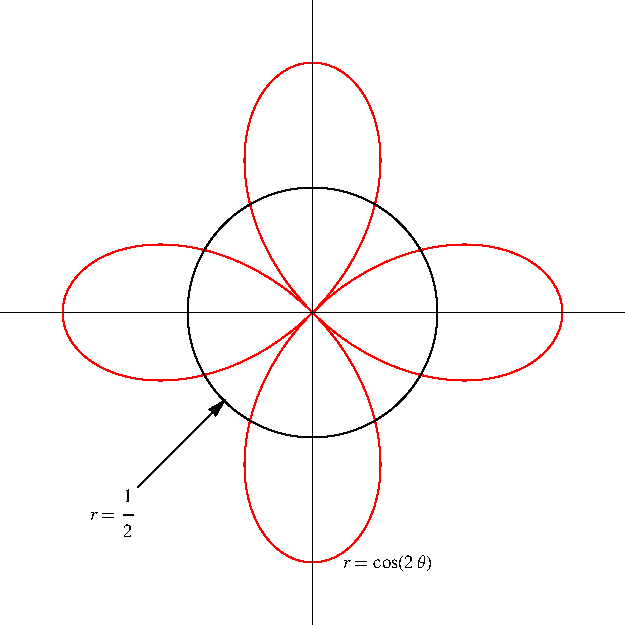
\includegraphics[height=5cm]{polar-curves/pictures/11-04-ex3a.pdf}%
%}%
%\only<handout:0| 4-5>{%
%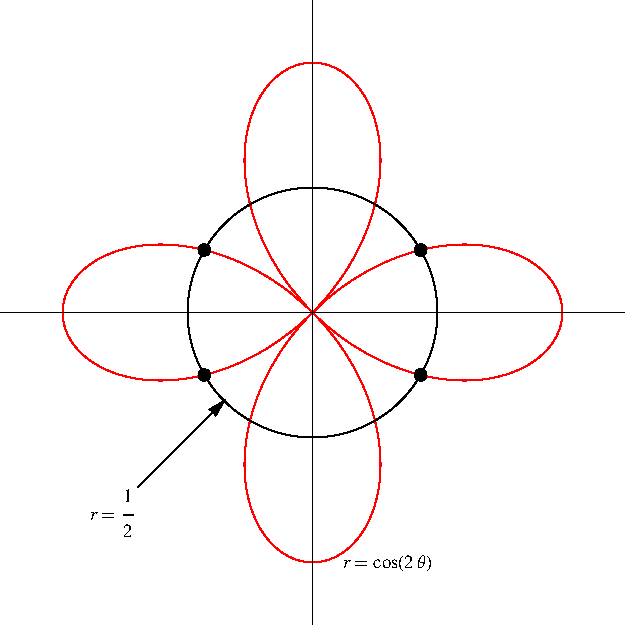
\includegraphics[height=5cm]{polar-curves/pictures/11-04-ex3b.pdf}%
%}%
%\only<6-8>{%
%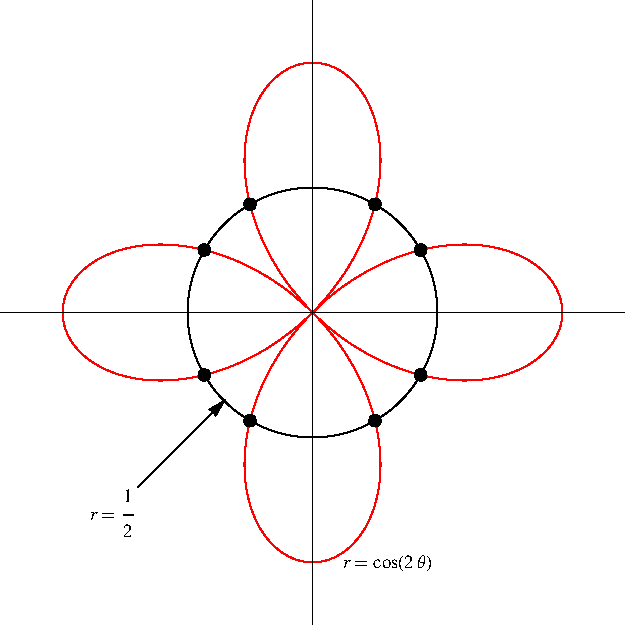
\includegraphics[height=5cm]{polar-curves/pictures/11-04-ex3c.pdf}%
%}%
%\only<handout:0| 9>{%
%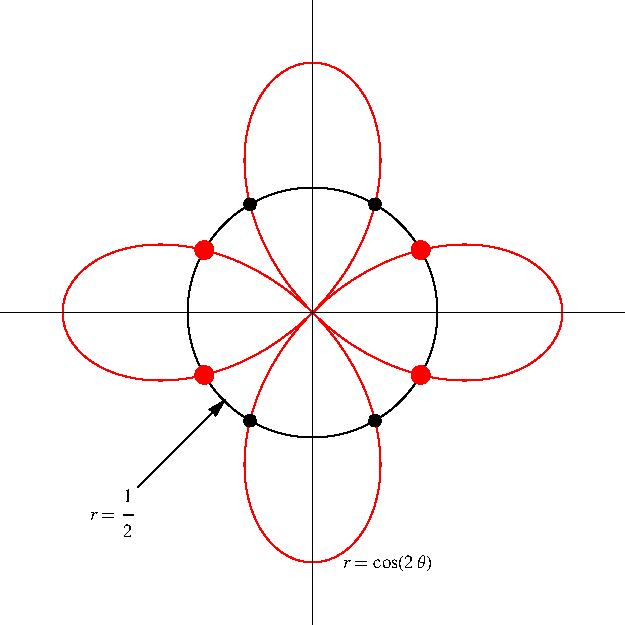
\includegraphics[height=5cm]{polar-curves/pictures/11-04-ex3d.pdf}%
%}%
%\only<handout:0| 10->{%
%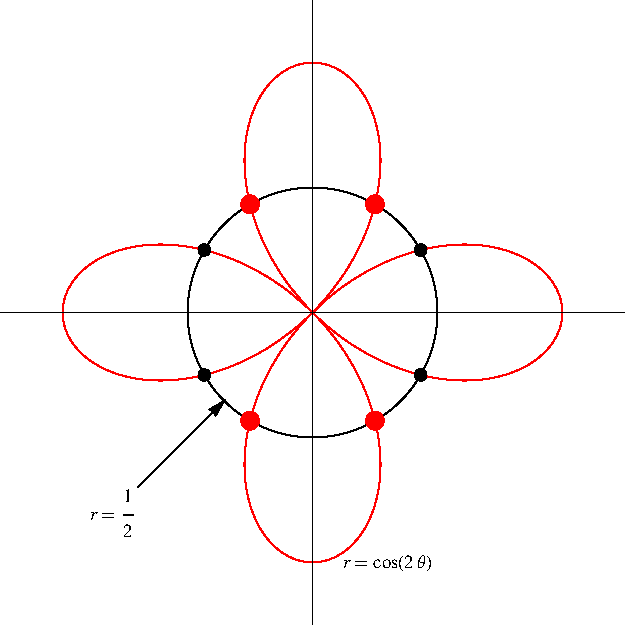
\includegraphics[height=5cm]{polar-curves/pictures/11-04-ex3e.pdf}%
%}%
\column{.6\textwidth}
\abovedisplayskip=0pt
\belowdisplayskip=0pt
\begin{eqnarray*}
\uncover<2->{%
\cos 2\theta%
}%
& \uncover<2->{ = } &%
\uncover<2->{%
\frac{1}{2}%
}\\%
\uncover<3->{%
2\theta%
}%
& \uncover<3->{ = } &%
\uncover<3->{%
\frac{\pi}{3}, \frac{5\pi}{3}, \frac{7\pi}{3}, \frac{11\pi}{3}%
}\\%
\uncover<4->{%
\theta%
}%
& \uncover<4->{ = } &%
\uncover<4->{%
\frac{\pi}{6}, \frac{5\pi}{6}, \frac{7\pi}{6}, \frac{11\pi}{6}%
}%
\end{eqnarray*}
\begin{itemize}
\item<5->  This only gives four points.
\item<6->  There are actually eight.
\item<7->  The circle $r = \frac{1}{2}$ also has polar equation $r = -\frac{1}{2}$.
\item<8->  To find all eight points, solve \alertNoH{ 9}{$\cos (2\theta )= \frac{1}{2}$} and \alertNoH{ 10}{$\cos (2\theta) = -\frac{1}{2}$}.
\end{itemize}
\end{columns}
\end{example}
\end{frame}
% end module polar-intersection-ex3


\section{Cylindrical Coordinates}
\begin{frame}
 \frametitle{Cylindrical coordinates}
\begin{columns}
\column{0.4\textwidth}
%
  \psfrag{P}{$P$}
  \psfrag{O}{$O$}  
  \psfrag{xp}{$x_P$} 
  \psfrag{yp}{$y_P$} 
  \psfrag{zp}{$z_P$}     
  \psfrag{rp}{$r_P$}
  \psfrag{thp}{$\theta_P$}
  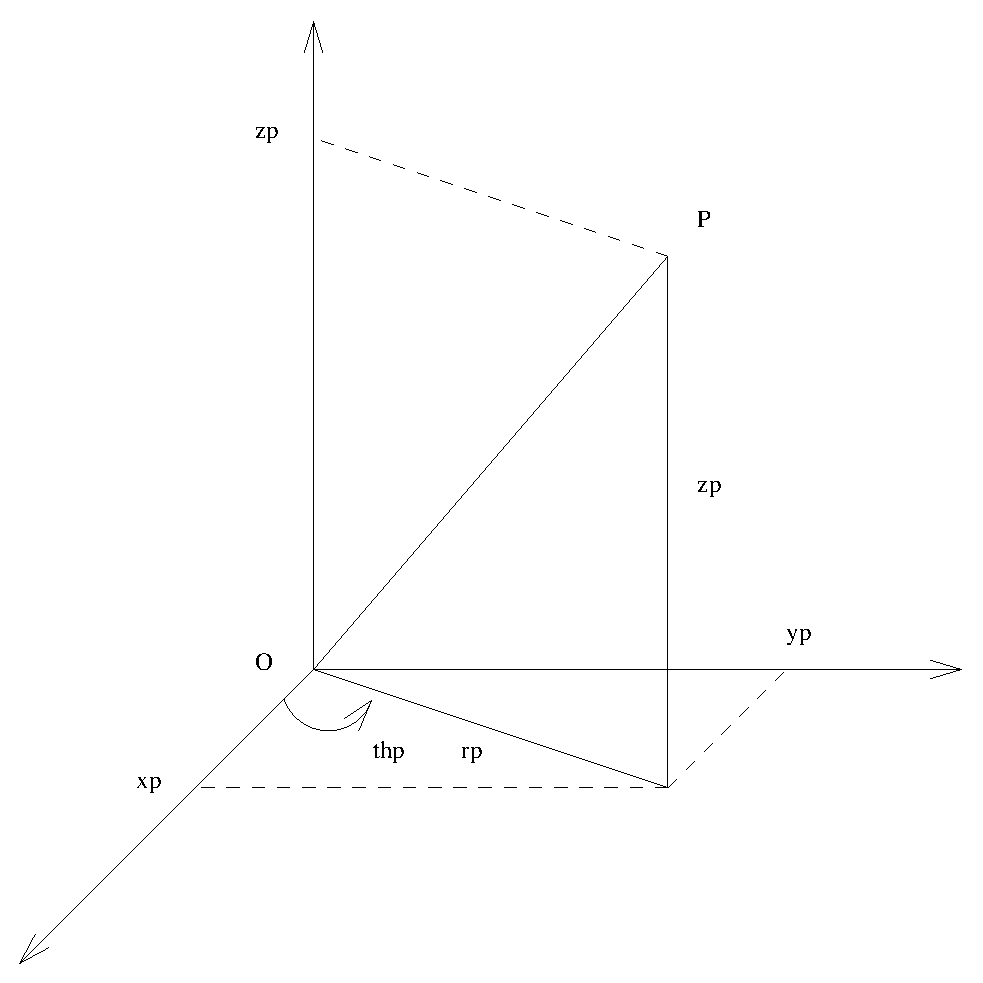
\includegraphics[height=2in]{../../modules/coordinate-systems/pictures/cylindrical_coordinates.eps}
  %\caption{Cylindrical coordinates}
  %\label{fig:cylindrical-coordinates}
%
\column{0.6\textwidth}
$$P(x,y,z) \Longleftrightarrow P(r, \theta, z)$$

\begin{itemize}
    \item Polar in $Oxy$ -- $(r, \theta)$;
    \item Rectangular in $Orz$ -- $(r, z)$.
\end{itemize}
\end{columns}

\end{frame}

\begin{frame}

\begin{columns}
\column{0.4\textwidth}
  \psfrag{P}{$P$}
  \psfrag{O}{$O$}  
  \psfrag{xp}{$x_P$} 
  \psfrag{yp}{$y_P$} 
  \psfrag{zp}{$z_P$}     
  \psfrag{rp}{$r_P$}
  \psfrag{thp}{$\theta_P$}
  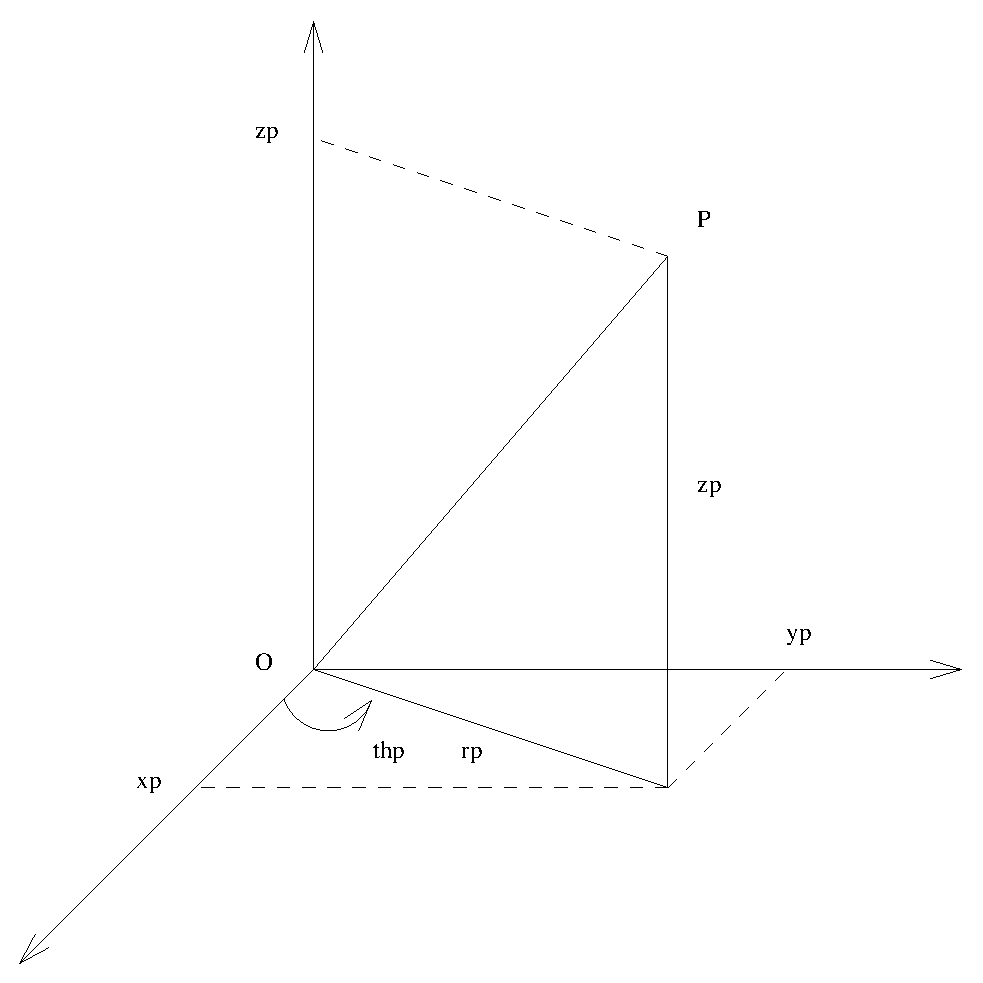
\includegraphics[height=2in]{../../modules/coordinate-systems/pictures/cylindrical_coordinates.eps}
  %\caption{Cylindrical coordinates}
  %\label{fig:cylindrical-coordinates}
%
\column{0.6\textwidth}
To transform cylindrical to rectangular coordinates:\pause
$$x=r\cos\theta \quad , \quad y = r\sin\theta \quad , \quad z_{r} = z_{c}$$

Rectangular to cylindrical:\pause
$$r= \sqrt{x^2+y^2} \quad , \quad z_{c}=z_{r}$$
$$\cos\theta = \frac{x}{r} \quad , \quad \sin\theta = \frac{y}{r}\; .$$
\end{columns}
\end{frame}

\begin{frame}
\frametitle{Constant Coordinate Sets}
\begin{columns}
\column{0.4\textwidth}
  \psfrag{P}{$P$}
  \psfrag{O}{$O$}  
  \psfrag{xp}{$x_P$} 
  \psfrag{yp}{$y_P$} 
  \psfrag{zp}{$z_P$}     
  \psfrag{rp}{$r_P$}
  \psfrag{thp}{$\theta_P$}
  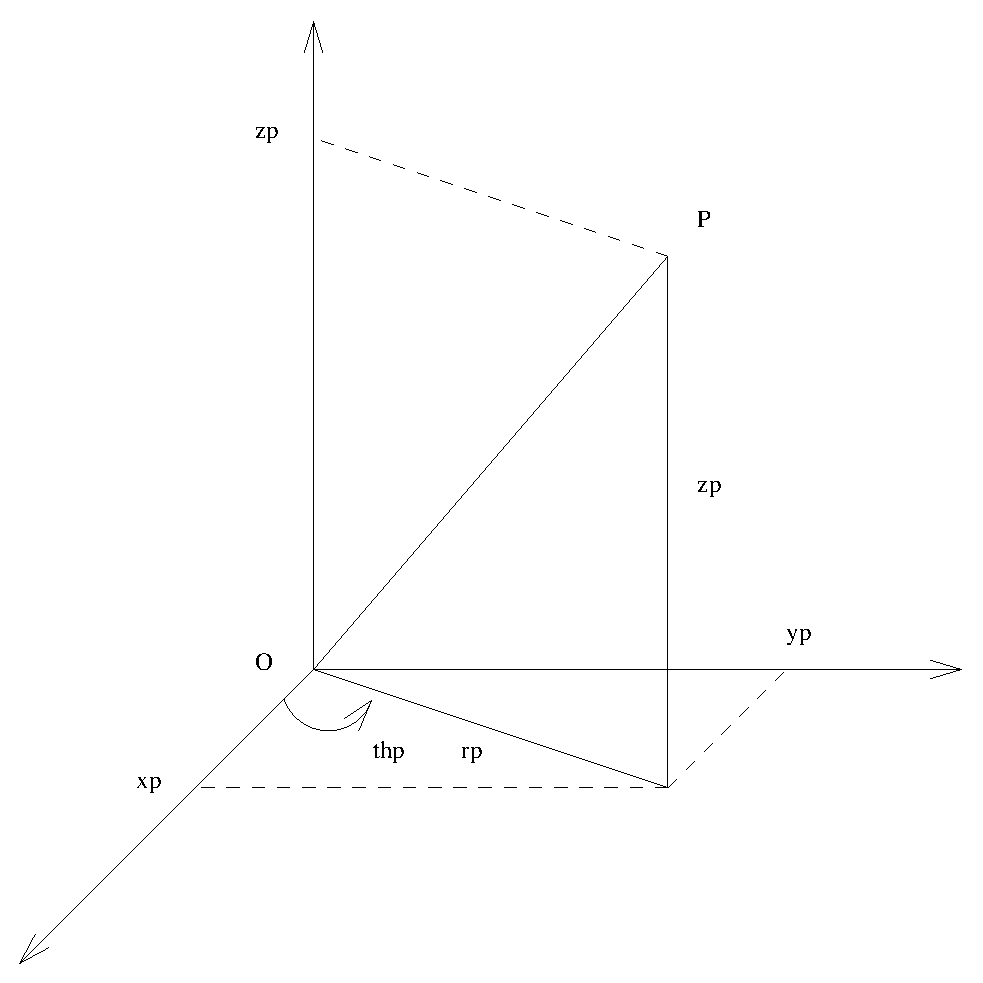
\includegraphics[height=2in]{../../modules/coordinate-systems/pictures/cylindrical_coordinates.eps}
\column{0.6\textwidth}

Surfaces:
\begin{itemize}
  \item $r$ constant \pause$\to$ vertical cylinder;
  \item $\theta$ constant \pause$\to$ vertical half plane;
  \item $z$ constant \pause$\to$ horizontal plane.\pause
\end{itemize}
%
Curves:
\begin{itemize}
 \item $\theta, z$ constant \pause$\to$ horizontal ray;
\item $r, z$ constant \pause$\to$ horizontal circle;
\item $r, \theta$ constant \pause$\to$ vertical line.
\end{itemize}
\end{columns}
\end{frame}
\section{Spherical Coordinates}
\begin{frame}
 \frametitle{Spherical Coordinates}
\begin{columns}
\column{0.55\textwidth}
%  \psfrag{P}{$P$}
%  \psfrag{O}{$O$}
%  \psfrag{xp}{$x_P$}
%  \psfrag{yp}{$y_P$}
%  \psfrag{zp}{$z_P$}
%  \psfrag{rho}{$\rho_P$}
%  \psfrag{thp}{$\theta_P$}
%  \psfrag{phi}{$\phi_P$}
\psset{xunit=1cm, yunit=1cm}
\begin{pspicture}(-2.1,-2.5)(5,5.2)
\tiny
\renewcommand{\fcScreen}{[-1 -0.4 -0.25] -1}
\fcBoundingBox{-2.1}{-2.5}{2}{2}
\fcAxesIIId{5}{5}{5}
\fcPutIIId[r]{[0 -0.15 0.15]}{$O$}
\fcLineIIId[linestyle=dotted]{[3 0 0]}{[3 3 0]}
\fcLineIIId[linestyle=dotted]{[3 3 0]}{[0 3 0]}
\fcLineIIId[linestyle=dotted]{[0 0 0]}{[0 3 0]}
\fcLineIIId{[0 0 0]}{[3 3 0]}
\fcLineIIId{[3 3 0]}{[3 3 3]}
\fcLineIIId{[0 0 3]}{[3 3 3]}
\fcPutIIId[l]{[3.1 3.1 3.1]}{$P$}
\fcPutIIId[r]{[1.5 -0.1 0]}{$x_P$}
\fcPutIIId[t]{[3 3 0]}{$Q$}
\fcPutIIId[b]{[0 1.5 0]}{$y_P$}
\fcPutIIId[l]{[3 3 1.5]}{$~~z_P$}
\fcPutIIId[r]{[0 0 1.5]}{$z_P~~$}
\uncover<2->{%
\fcLineIIId{[0 0 0]}{[3 3 3]}
\uncover<3>{\fcLineIIId[linecolor=red, linewidth=2pt]{[0 0 0]}{[3 3 3]}}%
\fcPutIIId[r]{[2.1 2.1 2.1]}{$\rho_P$}
\fcPutIIId[rt]{[1 1 1.5]}{$\phi_P~~$}
\fcPutIIId[tr]{[1.8 0.9 0]}{$\theta_P$}%
\fcAngleIIId[linecolor=red, arrows=->]{[0 0 1]}{[3 3 3]}{1.7}%
\uncover<4>{\fcAngleIIId[linecolor=red, linewidth=2pt, arrows=->]{[0 0 1]}{[3 3 3]}{1.7}}%
\fcAngleIIId[linecolor=red, arrows=->]{[1 0 0]}{[3 3 0]}{1.7}%
\uncover<5>{\fcAngleIIId[linecolor=red, arrows=->, linewidth=2pt]{[1 0 0]}{[3 3 0]}{1.7}}%
}%
\uncover<8>{\fcLineIIId[arrows=->, linecolor=red, linewidth=2pt]{[0 0 0]}{[5 5 5]}}%
\uncover<10>{%
\fcAngleIIId[linecolor=red, linewidth=2pt]{[0 0 1]}{[1 1 0]}{2}%
\fcAngleIIId[linecolor=red, linewidth=2pt, arrows=->]{[1 1 0]}{[0 0 -1]}{2}%
}%
\uncover<12>{%
\fcAngleIIId[linecolor=red, linewidth=2pt]{[1 0 0]}{[0 1 0]}{2}%
\fcAngleIIId[linecolor=red, linewidth=2pt]{[0 1 0]}{[-1 0 0]}{2}%
\fcAngleIIId[linecolor=red, linewidth=2pt]{[-1 0 0]}{[0 -1 0]}{2}%
\fcAngleIIId[linecolor=red, linewidth=2pt, arrows=->]{[0 -1 0]}{[1 0 0]}{2}%
}%
\end{pspicture}
%  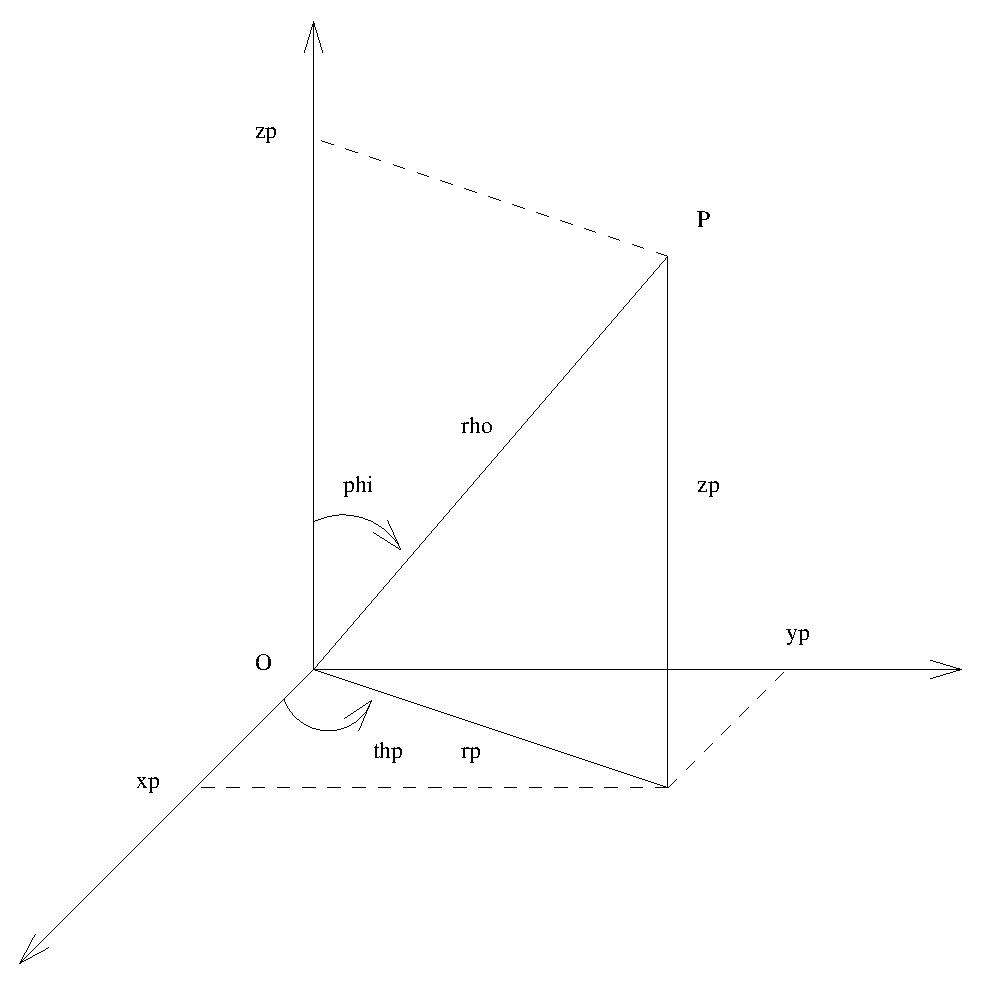
\includegraphics[height=2in]{../../modules/coordinate-systems/pictures/ok-cylindrical-spherical.eps}
\column{0.45\textwidth}
\begin{itemize}
\item In Cartesian coordinates, a point $P$ is given by triple $(x_P, y_P, z_P)$.
\item<2-> We introduce alternative spherical coordinates $(\rho_P, \phi_P,\theta_P)$.
\begin{itemize}
\item \alertNoH{3}{$\rho_P$: distance $|OP|$;}
\item \alertNoH{4}{$\phi_P$: angle $Oz$ to $OP$;}
\item \alertNoH{5}{$\theta_P$: angle $Ox$ to $OP_{xy}$.}
\end{itemize}
\item<6-> Coordinates range:
\begin{itemize}
\item \alertNoH{7,8}{$\rho$:} \uncover<8->{\alertNoH{8}{ $[0,\infty)$;}}
\item \alertNoH{9,10}{$\phi$:}  \uncover<10->{\alertNoH{10}{$[0, \pi]$;}}
\item \alertNoH{11,12}{$\theta$:}  \uncover<12->{ \alertNoH{12}{$[0,2\pi)$.}}
\end{itemize}
\end{itemize}
\end{columns}
\end{frame}

\begin{frame}
\frametitle{Transition Spherical - Rectangular coordinates}
\begin{columns}
\column{0.4\textwidth}
\psset{xunit=1cm, yunit=1cm}
\begin{pspicture}(-3,-2)(2,2)
\tiny
\renewcommand{\fcScreen}{[-1 -0.4 -0.25] -1}
\fcLineIIId[arrows=->]{[0 0 0]}{[5 0 0 ]}
\fcLineIIId[arrows=->]{[0 0 0]}{[0 5 0 ]}
\fcLineIIId[arrows=->]{[0 0 0]}{[0 0 5 ]}
\fcPutIIId[r]{[0 -0.15 0.15]}{\alert<2,3,4>{$O$}}
\fcLineIIId[linecolor=gray]{[3 0 0]}{[3 3 0]}
\fcLineIIId[linecolor=gray]{[3 3 0]}{[0 3 0]}
\fcLineIIId{[0 0 0]}{[3 3 0]}
\fcLineIIId{[3 3 0]}{[3 3 3]}
\fcLineIIId{[0 0 0]}{[3 3 3]}
\fcLineIIId{[0 0 3]}{[3 3 3]}
\fcPutIIId[l]{[3.1 3.1 3.1]}{\alert<4>{$P$}}
\fcPutIIId[r]{[1.5 -0.1 0]}{$\alert<1>{x}$}
\fcPutIIId[t]{[3.1 3.1 0]}{\alert<2,3>{$Q$}}
\uncover<2->{\fcPutIIId[l]{[1.4 1.5 0]}{\alert<4,5,6>{$~~r$}}}
\uncover<2->{
\fcPutIIId[r]{[3 -0.1 0]}{\alert<2,3>{$S$}}
\fcPolyLineIIId[linecolor=red]{[2.6 0 0 ] [2.6 0.4 0] [3 0.4 0]}
}
\uncover<2->{
\fcPutIIId[b]{[-0.1 1.5 0]}{$y$}
\fcPutIIId[t]{[3.1 1.5 0]}{\alert<5>{$y$}}
}
\uncover<7->{\fcPutIIId[r]{[0 0 1.5]}{\alert<7>{$z~~$}}}
\uncover<4->{
\fcPutIIId[r]{[0 -0.1 3]}{\alert<4>{$T~$}}
\fcPutIIId[b]{[1.4 1.5 3]}{\alert<4,6>{$~~r$}}
\fcPolyLineIIId[linecolor=red]{[2.6 2.6 0] [2.6 2.6 0.56569] [3 3 0.56569]}
\fcPolyLineIIId[linecolor=red]{[0.4 0.4 3] [0.4 0.4 3 0.56569 sub] [0 0 3 0.56569 sub]}
}
\fcPutIIId[r]{[1.7 1.7 1.7]}{\alert<4,6,7>{$\rho~~$}}
\fcPutIIId[rt]{[0.8 0.8 1.3]}{\alert<4,6,7>{$\phi~~$}}
\fcPutIIId[br]{[1.2 0.5 0]}{\alert<3,5>{$\theta$}}
\fcCurveIIId[linecolor=red, arrows=->]{0}{54.74}{ %
t sin 45 cos mul 1.5 mul % 
t sin 45 sin mul 1.5 mul %
t cos 1.5 mul %
} %
\fcCurveIIId[linecolor=red, arrows=->]{0}{45}{ %
t cos 1.5 mul % 
t sin 1.5 mul %
0 %
} %
\end{pspicture} 
\column{0.6\textwidth}

From spherical to rectangular coords:
\[
\begin{array}{rcll|l}
\alert<1->{x}&\alert<1>{=}& \uncover<3->{\alert<3>{ \alert<4>{r}\cos\theta}} &&\uncover<2->{\alert<2,5>{ \text{use }\triangle SQO}} \\ 
\uncover<4->{&\alert<0>{=} & \alert<4>{\rho\sin\phi }\cos\theta &&\alert<4,6,7>{ \text{use }\triangle OPT} }\\
\uncover<5->{\alert<5>{y}&\alert<0>{=}& \alert<5>{\alert<6>{r} \sin\theta } }\\
\uncover<6->{&\alert<0>{=}& \alert<6>{\rho\sin\phi }\sin\theta} \\
\uncover<7->{\alert<7>{z}&\alert<7>{=}& \alert<7>{\rho\cos\phi }}
\end{array}
\]
\uncover<8->{
From rectangular to spherical coords:
$$\rho = \sqrt{x^2+y^2+z^2} \quad , \quad r = \sqrt{x^2+y^2}$$
$$\cos\phi = \frac{z}{\rho} \quad , \quad \sin\phi = \frac{r}{\rho}$$
$$\cos\theta = \frac{x}{r} \quad , \quad \sin\theta = \frac{y}{r}$$
}
\end{columns}
\end{frame}

\begin{frame}
 \frametitle{Curvilinear boxes}
 
 Polar ``wedge'':
 %
$$C  = \{ P(r,\theta) \; | \;r_0 \leqslant
r \leqslant r_0+\Delta r,  \theta_0 \leqslant \theta
\leqslant \theta_0+\Delta \theta\} \; .$$
%
Shape? \pause Area = ...?
\pause

\bigskip

Cylindrical ``box'':
%
$$X = \{ P(r,\theta, z) \; | \; 0 \leqslant r \leqslant r_0\, ,
0 \leqslant \theta \leqslant \theta_0\, ,
0 \leqslant z \leqslant z_0\}$$

\pause
Shape ? \pause Volume = ...?

\bigskip

\pause
Spherical ``box'':
%
$$Y = \{ P(\rho, \phi, \theta) \; | \; 0 \leqslant \rho \leqslant \rho_0\, ,
0 \leqslant \phi \leqslant \phi_0\, ,
0 \leqslant \theta \leqslant \theta_0\}$$

\pause
Shape? \pause Volume = ...?

\end{frame}
}% end lecture


% begin lecture

%\section{(Appendix G) Complex Numbers}
% WARNING:  Appendix G is missing here.
% end lecture
\end{document}
